\section{Formulation} \label{sec:formul}
The phase-field model as a diffuse interface model does not introduce discontinuities into the solid but the fracture surface is approximated by a scalar valued field. Thus, the boundary between damaged and not damaged areas is smoothed. In the following parts, a model for brittle and ductile fracture as well as a second- and fourth-order model are presented. At first, the notation and formulation considering brittle fracture is outlined. Afterwards, differences in the formulation considering ductile fracture are shown. For the rest of this paper, following notation is made (see \figref{fig:bodies}\subrefnew{fig:body_1}). The arbitraray body $\Omega\subset\mathbb{R}^{d}$ ($d\in\{1,2,3\}$) has external boundary $\partial\Omega$ and evolving internal discontinuity boundary (fracture surface) $\Gamma$. The displacement field at a given point $\mathbf{x}$ and time $t$ is given by $\mathbf{u}\left(\mathbf{x},t\right)\in\mathbb{R}^{d}$. Dirichlet boundary conditions $\mathbf{u}\left(\mathbf{x},t\right)=\mathbf{g}\left(\mathbf{x},t\right)$ on $\partial\Omega_{\mathbf{g}}$ and Neumann boundary conditions $\mathbf{t}\left(\mathbf{x},t\right)=\mathbf{h}\left(\mathbf{x},t\right)$ on $\partial\Omega_{\mathbf{h}}$ are imposed with $\partial\Omega_{\mathbf{g}}\cup\partial\Omega_{\mathbf{h}}=\partial\Omega$. $\mathbf{t}\left(\mathbf{x},t\right)$ describes a given traction vector force.
\begin{figure}[ht!]
    \centering
    \begin{subfigure}[t]{0.4\textwidth}
        \centering
        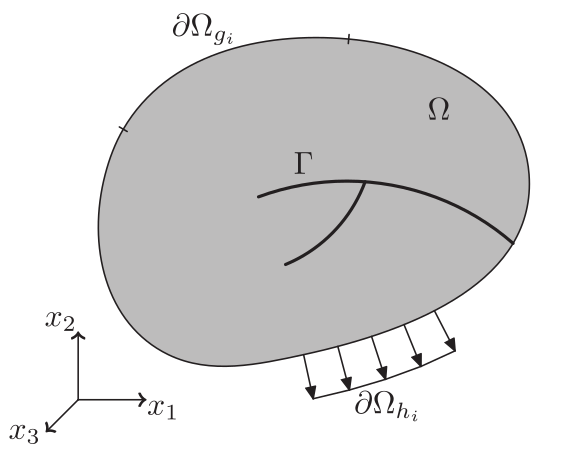
\includegraphics[scale=0.3]{data/Body_1}
        \caption{}\label{fig:body_1}
    \end{subfigure}
    %
    \begin{subfigure}[t]{0.5\textwidth}
        \centering
        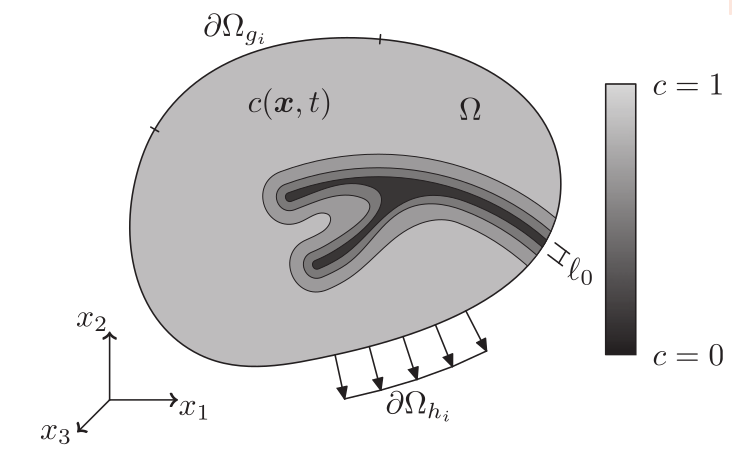
\includegraphics[scale=0.3]{data/Body_2}
        \caption{}\label{fig:body_2}
    \end{subfigure}
    \caption{\subrefnew{fig:body_1} Representation of a solid body $\Omega$ and internal discontinuitiy boundary $\Gamma$. \subrefnew{fig:body_2} Phase-field approximation of $\Gamma$. $c\left(\mathbf{x},t\right)$ describes the phase-field and $l_{0}$ is a parameter for controlling the failure zone's width. \cite{01_PF_dyn_brittle}} \label{fig:bodies}
\end{figure}


\subsection{Griffith's theory of brittle fracture} \label{sec:formul_Griffith}
Considering small derformations and deformation gradients, the small strain tensor $\bm{\varepsilon}\left(\mathbf{x},t\right)$ is given by
\begin{equation}
	\bm{\varepsilon} = \nabla^{s}\mathbf{u}
\end{equation}
where $\left(\cdot\right)^{s}$ refers to the symmetric part. Considering isotropic linear elasticity, the undamaged elastic energy densitiy can be expressed by
\begin{equation} \label{eq:psi_e}
	\Psi_ {e}\left(\bm{\varepsilon}\right) = \dfrac{1}{2}\lambda tr\left(\bm{\varepsilon}\right)^{2}+\mu\bm{\varepsilon}:\bm{\varepsilon}
\end{equation}
using the Lam\'{e} constants $\lambda$ and $\mu$ and $\left(\cdot\right):\left(\cdot\right)$ denoting the double contraction.

According to the energetic approaches to fracture, the critical fracture energy density $\mathcal{G}_{c}$ defines the energy being necessary to create a unit area of fracture surface. Since translation of cracks shall be forbidden and extension, branching and merging shall be allowed, there is an irreversibility condition stating $\Gamma\left(t\right)\subseteq\Gamma\left(t+\Delta t\right), \forall \Delta t>0$.

However, Griffith's fracture theory reaches its limits as soon as it is used to predict crack paths, nucleation of new cracks, complicated crack behaviours during kinking and branching. Thus, the problem is formulated in a variational sense which is shown in the following paragraphs. The phase-field approach can then be seen as a regularized version of this variational formulation. \citep{05_PF_ductile}

Newton's laws follow Hamilton's principle stating that the functional 
\begin{equation} \label{eq:fctal_Hamilton}
	J\left(q,\dot{q}\right)=\int\limits_{t_{0}}^{t_{1}}\mathcal{L}\left(q,\dot{q},t\right)\mathrm{d}t
\end{equation} reaches a stationary point. $\mathcal{L}\left(q,\dot{q},t\right)$ describes the so called Lagrangian and $q$ represents generalized coordinates. The motion of the mechanical system from $t_{0}$ to $t_{1}$ is then captured by this formulation \citep{01_B_LagrMech}. In our case, the Lagrangian reads $\mathcal{L}\left(\mathbf{u},\dot{\mathbf{u}},\Gamma\right)=\Psi_{kin}\left(\mathbf{u}\right)-\Psi_{pot}\left(\mathbf{u},\Gamma\right)$. Inserting the introduced cricical fracture energy densitiy $\mathcal{G}_{c}$, the kinetic energy of the body and \eqref{eq:psi_e} leads to
\begin{equation} \label{eq:lagr}
	\mathcal{L}\left(\mathbf{u},\dot{\mathbf{u}},\Gamma\right) = \int\limits_{\Omega}\left(\frac{1}{2}\rho\dot{\mathbf{u}}\dot{\mathbf{u}}-\Psi_{e}\left(\bm{\varepsilon}\right)\right)\mathrm{d}\Omega - \int\limits_{\Gamma}\mathcal{G}_{c}\mathrm{d}\Gamma.
\end{equation}
The Euler-Lagrange Equation (ELE) is a differential equation which solution satisfies equilibrium. Thus, this equation is also called the equation of motion \footnote{The term \textit{equation of motion} may be a bit misleading. It refers to the differential equation and not to its solution.}. A minimizer $q$ for \eqref{eq:lagr} satisfies the ELE
\begin{equation} \label{eq:ELE_O2}
	\dfrac{\partial\mathcal{L}}{\partial q}-\dfrac{\mathrm{d}}{\mathrm{d}t}\dfrac{\partial\mathcal{L}}{\partial\dot{q}}=0.
\end{equation}
For a given $\mathcal{L}=\mathcal{L}\left(q,\dot{q},\ddot{q}, t\right)$ this differential equation is changed to
\begin{equation} \label{eq:ELE:_O4}
	\dfrac{\partial\mathcal{L}}{\partial q}-\dfrac{\mathrm{d}}{\mathrm{d}t}\dfrac{\partial\mathcal{L}}{\partial\dot{q}}+\dfrac{\mathrm{d}^{2}}{\mathrm{d}t^{2}}\dfrac{\partial\mathcal{L}}{\partial\ddot{q}}=0
\end{equation}
\citep{01_B_LagrMech}. So as to circumvent problems of algorithmically tracking the propagating dicontinuity $\Gamma$, the phase-field approach will be presented in the next chapters which regularizes the just mentioned variational formulation.

\subsection{Phase-field approximation} \label{sec:ph_approx}
As can be seen in \figref{fig:bodies}\subrefnew{fig:body_2} the fracture surface $\Gamma$ is approximated by a scalar valued field $c\left(\mathbf{x},t\right)$. This field is called the phase-field. Values of $c=1$ represent regions away from the crack (undamaged material) whereas $c=0$ symbolizes the crack. Now, in \eqref{eq:lagr} the surface integral and thus, the need for tracking the crack can be eliminated. The approximation reads as follows:
\begin{equation} \label{eq:surf_int_approx}
	\int\limits_{\Gamma}\mathcal{G}_{c}\mathrm{d}\Gamma \approx \int\limits_{\Omega}\mathcal{G}_{c}\Gamma_{c,n}\mathrm{d}\Omega.
\end{equation}
Obviously, the surface integral can now be approximately calculated without knowing or tracking the fracture surface. \eqref{eq:surf_int_approx} represents the fracture surface energy. The quantity $\Gamma_{c,n}$ is called the crack density functional which depends on a parameter $l_{0}$, the phase-field $c\left(\mathbf{x},t\right)$ and its spatial derivatives up to order $\frac{n}{2}$ ($\frac{\partial c}{\partial \mathbf{x}},..,\frac{\partial^{\frac{n}{2}} c}{\partial \mathbf{x}^{\frac{n}{2}}}$). $l_{0}\in\mathbb{R}^{+}$ represents a parameter controlling the width of the approximation of the crack (see \figref{fig:bodies}\subrefnew{fig:body_2}). It could be seen as a numerical regularization parameter or as an material parameter. \citet{01_PF_dyn_brittle} showed that a critical stress level $\sigma_{c}$ depends on $l_{0}$. Thus, this parameter is here seen as a material property. For a more detailed discussion it refered to the investigations of \citet{07_PF_l0}.

The notation $\Gamma_{c,n}$ already presages that $n$ determines the order of the approximation. \citet{02_PF_HO_brittle} presented a so called \textit{second-} and \textit{fourth-order phase-field theory}. For $n=2$ the crack density functional introduced by \citet{08_PF_Gammac2} is used where as for $n=4$ a new functional has been established:
\begin{align}
	\begin{aligned}   \label{eq:crack_dens_fctals}
		\Gamma_{c,2} &= \dfrac{1}{4l_{0}}\left[\left(c-1\right)^{2}+4l_{0}^{2}|\nabla c|^{2}\right], \\
		\Gamma_{c,4} &= \dfrac{1}{4l_{0}}\left[\left(c-1\right)^{2}+2l_{0}^{2}|\nabla c|^{2}+l_{0}^{4}\left(\Delta c\right)^{2}\right].
	\end{aligned}
\end{align}
These formulations have been analytically analysed. So as to keep things short, it is referred to the work by \citet{02_PF_HO_brittle} for more detailed information. Only one important aspect is mentioned here: ${\eqref{eq:crack_dens_fctals}}_{1}$ is well-posed variationally for all $c\in H^{1}\left(\Omega\right)$ and solutions will generally not show greater regularity. Thus, ${\eqref{eq:crack_dens_fctals}}_{2}$ has been introduced so as to provide higher regularity in the solutions.

\subsection{Energy approximation} \label{sec:energy_approx}
In the failure zone there is a loss of material stiffness. So as to model this phenomena the elastic energy is split into contributions from tensile and compressive deformations\footnote{Originally, a parameter $k$ or $\eta<<1$ has been introduced by \citet{09_PF_k} into this equation so as to avoid ill-posedness. However, \citet{01_PF_dyn_brittle} found out that there is no necessity of setting $k>0$. Thus, the derivation of the governing evolution equations all include that $k=0$.}
\begin{equation} \label{eq:el_energy}
	\Psi_{e}\left(\bm{\varepsilon},c\right)=g\left(c\right) \Psi_{e}^{+}\left(\bm{\varepsilon}\right)+\Psi_{e}^{-}\left(\bm{\varepsilon}\right)
\end{equation}
with the so called degradation function $g\left(c\right)=c^{2}$. At a later point in this work there will be more information on this function. This splitting is achieved with the help of spectral decomposition of the strain:
\begin{align} \label{eq:spectr_decomp}
	\begin{aligned}
		\bm{\varepsilon} = \mathbf{P}\bm{\Lambda}\mathbf{P}^{T} \quad \Rightarrow \quad \bm{\varepsilon}^{+} = \mathbf{P}\bm{\Lambda}^{+}\mathbf{P}^{T},  \bm{\varepsilon}^{-} = \mathbf{P}\bm{\Lambda}^{-}\mathbf{P}^{T}, \\
		\bm{\Lambda}^{+}=diag\left(\left<\lambda_{1}\right>,\left<\lambda_{2}\right>,\left<\lambda_{3}\right>\right), \quad \left<x\right>=\begin{cases}x, &x>0 \\ 0, & x\leq0\end{cases}.
	\end{aligned}
\end{align}
$\bm{\Lambda}^{-}$ is analogously                                                                                                                                                                                                                                                                                                                                                                                                                                                                                                          defined. $\lambda_{i}\in\sigma\left(\bm{\varepsilon}\right),i\in\{1,2,3\}$ denote the eigenvalues of the strain tensor. Plugging \eqref{eq:spectr_decomp} into \eqref{eq:psi_e} leads to the energy contributions from tensile and compressive deformations:
\begin{align} \label{eq:psi_e+-}
	\begin{aligned}
		\Psi_{e}^{+}\left(\bm{\varepsilon}\right) &= \dfrac{1}{2}\lambda\left<tr\left(\bm{\varepsilon}\right)\right>^{2}+\mu tr\left[\left(\bm{\varepsilon}^{+}\right)\right], \\
		\Psi_{e}^{-}\left(\bm{\varepsilon}\right) &= \dfrac{1}{2}\lambda\left(tr\left(\bm{\varepsilon}\right)-\left<tr\left(\bm{\varepsilon}\right)\right>\right)^{2}+\mu tr\left[\left(\bm{\varepsilon}-\bm{\varepsilon}^{+}\right)\right].
	\end{aligned}
\end{align}
Putting \eqref{eq:el_energy} and \eqref{eq:surf_int_approx} together leads to the Helmholtz free energy given by
\begin{equation} \label{eq:Helmholtz}
	\Psi_{n}=c^{2}\Psi_{e}^{+}+\Psi_{e}^{-}+\mathcal{G}_{c}\Gamma_{c,n}.
\end{equation}

\subsection{Strong form} \label{sec:strong_form}
The governing equations will be one for enforcing stress equilibrium and the other will govern the phase-field evolution.

Assuming given body forces $\mathbf{b}$ and traction vector forces $\mathbf{t}=\bm{\sigma}\mathbf{n}$ with outward-pointing normal vector on $\partial\Omega$, stress equilibrium is enforced by
\begin{equation} \label{eq:stress_equil}
	 \left\{\begin{alignedat}{2}
\nabla\cdot\bm{\sigma}+\mathbf{b} &= \rho\ddot{\mathbf{u}} && \quad\text{on } \Omega\times\left(0,T\right) \\
		\mathbf{u} &= \mathbf{g} && \quad\text{on } \partial\Omega_{\mathbf{g}}\times\left(0,T\right) \\
		\bm{\sigma}\mathbf{n} &= \mathbf{h} && \quad\text{on } \partial\Omega_{\mathbf{h}}\times\left(0,T\right) \\
		\mathbf{u} &= \mathbf{u}_{0} && \quad\text{on } \Omega\times0 \\
		\dot{\mathbf{u}} &= \mathbf{v}_{0} && \quad\text{on } \Omega\times0.
  \end{alignedat}\right.
\end{equation}
$\eqref{eq:stress_equil}_{1}$ represents the local form of the linear momentum balance with $\bm{\sigma}=c^{2}\frac{\partial\Psi_{e}^{+}}{\partial\bm{\varepsilon}}+\frac{\partial\Psi_{e}^{-}}{\partial\bm{\varepsilon}}$.

As described in \secref{sec:formul_Griffith}, the Euler-Lagrange Equation can be used to find a minimizer of \eqref{eq:fctal_Hamilton}. Plugging \eqref{eq:crack_dens_fctals} and \eqref{eq:el_energy} into \eqref{eq:lagr} as well as using \eqref{eq:surf_int_approx} makes the use of the ELE possible. For this case, $q\hat{=}c$ and $\frac{\mathrm{d}}{\mathrm{d}t}\hat{=}\frac{\mathrm{d}}{\mathrm{d}\mathbf{x}}$. All this together lead to the governing equations for the evolution of the phase-field, namely $\eqref{eq:c2_equil}_{1}$ for the second- and $\eqref{eq:c4_equil}_{1}$ for the fourth-order phase-field theory. As can be seen in these equations, $\Psi_{e}^{+}$ has been replaced by strain histroy field $\mathcal{H}$ enforcing the irreversibility condition $\Gamma\left(t\right)\subseteq\Gamma\left(t+\Delta t\right), \forall \Delta t>0$ in the strong form. This field satisfies the Kuhn-Tucker conditions for loading and unloading \cite{01_PF_dyn_brittle}:
\begin{equation} \label{eq:KuhnTucker}
	\Psi_{e}^{+}-\mathcal{H}\leq0, \quad \dot{\mathcal{H}}\geq0, \quad \dot{\mathcal{H}}\left(\Psi_{e}^{+}-\mathcal{H}\right)=0.
\end{equation}
It can also be used to model pre-existing cracks or geometrical features \cite{01_PF_dyn_brittle}.

 \hl{\text{Boundary-Conditions!}}
\begin{equation} \label{eq:c2_equil}
		 \left\{\begin{alignedat}{2}
\left(\frac{4l_{0}\mathcal{H}}{\mathcal{G}_{c}}+1\right)c - 4l_{0}^{2}\Delta c=1 &= \rho\ddot{\mathbf{u}} && \quad\text{on } \Omega\times\left(0,T\right) \\
\hl{\nabla c\cdot\mathbf{n}} &= 0 && \quad \text{on } \partial\Omega\times\left(0,T\right) \\
\mathcal{H} &= \mathcal{H}_{0} && \quad \text{on } \Omega\times0  
\end{alignedat}\right.
\end{equation}
\begin{equation} \label{eq:c4_equil}
		 \left\{\begin{alignedat}{2}
\left(\frac{4l_{0}\mathcal{H}}{\mathcal{G}_{c}}+1\right)c - 2l_{0}^{2}\Delta c + l_{0}^{4}\Delta\left(\Delta c\right)=1 &= \rho\ddot{\mathbf{u}} && \quad\text{on } \Omega\times\left(0,T\right) \\
\hl{\Delta c} &= 0 && \quad \text{on } \partial\Omega\times\left(0,T\right) \\
\hl{\nabla\left(l_{0}^{4}\Delta c-2l_{0}^{2}c\right)\cdot\mathbf{n}} &= 0 && \quad \text{on } \partial\Omega\times\left(0,T\right) \\
\mathcal{H} &= \mathcal{H}_{0} && \quad \text{on } \Omega\times0  
\end{alignedat}\right.
\end{equation}
The numerical approximation of the solution of \eqref{eq:c2_equil} and \eqref{eq:c4_equil} are outlined in \secref{sec:num_formul}. The last topic of the next section is the difference in modelling ductile fracture in contrast to brittle fracture which has been considered up to this point.

\subsection{Ductile fracture} \label{sec:ductile_frac}
So as to motivate this section, at first the differences between the modelling of brittle and ductile fracture are examined. Up to this point of this paper, linear elasticity has been assumed. In this context, brittle fracture has been formulated in a variational way. By introducing the phase-field approximation, a regularized formulation of the variational one has been established. The corresponding stress-strain-curves and the procedure are illustrated in \figref{fig:elastic}.
\begin{table}[!ht]
	\begin{center}
	\begin{tabular}{|c||c|c|c|}
		\cline{2-4}
			\multicolumn{1}{c||}{}& Linear elasticity & \multicolumn{2}{c|}{Brittle fracture} \\
 		\hline\hline
			\rotatebox[origin=c]{90}{ Process} & \raisebox{-.5\height}{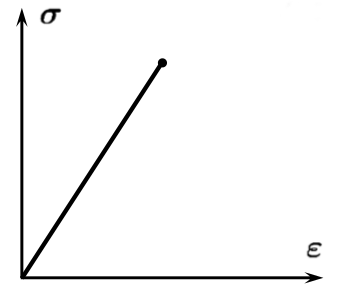
\includegraphics[scale=0.3]{data/elastic_1}} & \raisebox{-.5\height}{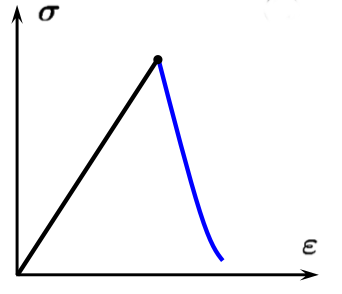
\includegraphics[scale=0.3]{data/elastic_2}} & \raisebox{-.5\height}{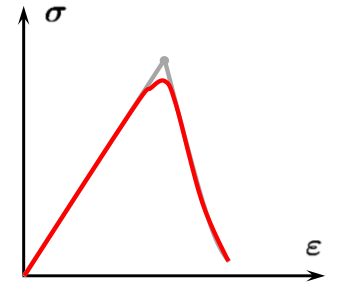
\includegraphics[scale=0.3]{data/elastic_3}} \\
		\hline
			\rotatebox[origin=c]{90}{\small{ Formulation }} & $E\left(\mathbf{u}\right)$ & \begin{tabular}[c]{@{}c@{}}Variational formulation\\of brittle fracture\\$E\left(\mathbf{u},\Gamma\right)$\end{tabular}  & \begin{tabular}[c]{@{}c@{}}Phase-field formulation\\($\hat{=}$regularized version)\\$E\left(\mathbf{u},c\right)$\end{tabular} \\
		\hline
	\end{tabular}
	\end{center}
\captionof{figure}{Brittle fracture: Process from linear elasticity over the variational formulation towards the phase-field approximation. \cite{06_PF_ductile}} \label{fig:elastic}
\end{table}
The variational formulation has been well established. Thus, the regularized version using the phase-field approximation could be found. As the dashed lines in \figref{fig:plastic} reveal, there is no variational formulation of ductile fracture found yet. Thus, the foundation of the regularized version is not as easy as for brittle fracture.

\begin{table}
	\begin{center}
	\begin{tabular}{|c||c|c|c|}
		\cline{2-4}
			\multicolumn{1}{c||}{}& Plasticity & \multicolumn{2}{c|}{Ductile fracture} \\
 		\hline\hline
			\rotatebox[origin=c]{90}{ Process} & \raisebox{-.5\height}{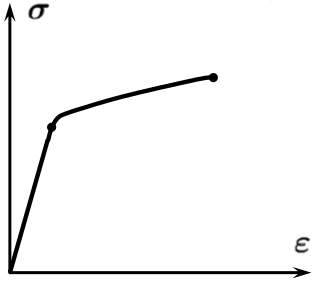
\includegraphics[scale=0.3]{data/plastic_1}} & \raisebox{-.5\height}{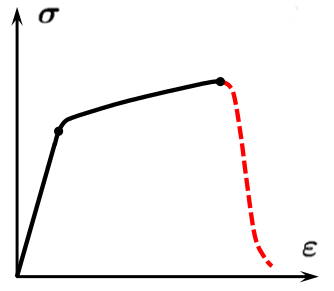
\includegraphics[scale=0.3]{data/plastic_2}} & \raisebox{-.5\height}{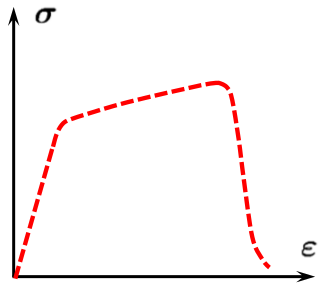
\includegraphics[scale=0.3]{data/plastic_3}} \\
		\hline
			\rotatebox[origin=c]{90}{\small{ Formulation }} & $E\left(\bm{\varepsilon}^{e},\bm{\varepsilon}^{p},\alpha\right)$ & \begin{tabular}[c]{@{}c@{}}Variational formulation\\of ductile fracture\\$E\left(\bm{\varepsilon}^{e},\bm{\varepsilon}^{p},\alpha,\Gamma\right)$\end{tabular}  & \begin{tabular}[c]{@{}c@{}}Phase-field formulation\\($\hat{=}$regularized version)\\$E\left(\bm{\varepsilon}^{e},\bm{\varepsilon}^{p},\alpha,c\right)$\end{tabular} \\
		\hline
	\end{tabular}
	\end{center}
\captionof{figure}{Ductile fracture: Process from plasticity towards the phase-field approximation. The variational formulation has not been established yet. \cite{06_PF_ductile}} \label{fig:plastic}
\end{table}


\hl{TODO}